\section{Theorie}

In dem folgenden Versuch soll die Molwärme von Kupfer bestimmt werden. Dabei wird
am Anfang auf verschiedene Modelle zur Erklärung der Molwärme bzw. derer verschiedenen
Abhängigkeite. Dafür werden nacheinander das klassische Modell, das Einstein-Modell
sowie das Debye-Modell besprochen. Die mit der Messung bestimmte Debye-Temperatur
$\theta\ua{D}$ wird dann abschließend mit dem errechneten Wert aus dem Debye-Ansatz
verglichen.

\subsection{Das klassische Modell}

Nach dem Äquipartitionsprinzip wird die einem Körper zugeführte Wärmemenge
gleichmäßig auf alle Bewegungsfreiheitsgrade der Atome verteilt. Die mittlere
Energie eines einzelnen Atoms beträgt dabei $\frac{1}{2}k\ua{B}T$. Die Atome in
einem Festkörper sind an festen Gitterplätzen lokalisiert, um die sie eine Schwingung
in drei senkrecht aufeinander stehende Richtungen ausführen können. Da bei harmonischen
Schwingungen die potentielle Energie gleich der kinetischen Energie ist, ergibt
sich für ein Atom die mittlere Energie
\begin{equation}
  \langle u \rangle = 3 k\ua{B} T.
\end{equation}
Für einen Mol eines Stoffes ergibt sich somit die Energie
\begin{equation}
  U = 3 k\ua{B} N\ua{L} T = 3 RT,
\end{equation}
wobei es sich bei $R$ um die allgemeine Gaskonstante und bei $N\ua{L}$ um die
Loschmidtsche Zahl handelt. Um die Molwärme bei konstantem Volumen zu erhalten,
muss die Energie nach der Temperatur abgeleitet werden. Für die spezifische Molwärme
erhält man somit den konstanten Wert
\begin{equation}
  C\ua{V} = \frac{\partial \su{U}}{\partial \su{T}}\ua{V} = 3R.
  \label{eqn:CVKlassisch}
\end{equation}
In der klassichen Theorie ergibt sich also keine Temperatur- oder Materialspezifische
Abhängigkeit. Dies steht im Widerspruch zu der beobachteten Abnahme der Molwärme
mit Abnahme der Temperatur, beschreibt die Molwärme aber zutreffend bei hohen Temperaturen
($T >> \theta\ua{D}$, Dulong-Petitsches Gesetz).

\subsection{Einstein-Modell}

Im Gegensatz zum klassischen Modell wird im Einstein-Modell die Quantelung der Energien
beachtet. Es wird angenommen, dass jedes Atom eine Schwingung mit der selben Frequenz
$\omega$ ausführt, wobei nur Energien als ganzzahlige Vielfache von $\hbar\omega$
aufgenommen oder abgegeben werden können. Die relative Wahrscheinlichkeit, dass ein
Oszillator im Gleichgewicht bei der Temperatur T die Energie $n\hbar\omega$ besitzt
ist durch die Boltzmann-Verteilung gegeben:
\begin{equation}
  W(n) = \exp {(-\frac{n\hbar\omega}{k\ua{B}T})}.
\end{equation}
Summiert man über alle möglichen Energien von $n=0$ bis $n=\infty$ multipliziert
mit der zugehörigen Wahrscheinlichkeit $W(n)$ und teilt dies durch die Summe aller
$W(n)$, erhält man die mittlere Energie eines Atoms:
\begin{equation}
  \langle u \rangle\ua{Einstein} = \frac{\hbar\omega}{\exp{(\sfrac{\hbar\omega}{k\ua{B}T})-1}}.
\end{equation}
Für die Molwärme erhält man dann analog zu \eqref{eqn:CVKlassisch} die Molwärme:
\begin{equation}
  C\ua{V, Einstein} = 3R \,\frac{\hbar^2\omega^2}{k\ua{B}^2T^2} \,\frac{\exp{(\sfrac{\hbar\omega}{k\ua{B}T})}}{\{\exp{(\frac{\hbar\omega}{k\ua{B}T})}-1\}^2}
\end{equation}
Für hohe Temperaturen ($k\ua{B}T>>\hbar\omega$) erhält man hier ebenfalls ein
asymptotisches Verhalten mit
\begin{equation}
  \lim\limits_{T \rightarrow \infty}{C\ua{V,Einstein}} = 3R.
\end{equation}
Im Gegensatz zum klassischen Modell wird hier somit die Abnahme der Molwärme mit
abnehmender Temperatur beschrieben. Jedoch zeigen sich insbesondere bei tiefen
Temperaturen Abweichungen zur ecperimentellen Kurve.

\subsection{Debye-Modell}

Im Debye-Modell wird im Gegensatz zum Einstein-Modell beachtet, dass die verschiedenen
Atome mit unterschiedlichen Frequenzen $\omega$ schwingen. Statt der singulären
Einstein-Frequenz wird hier die spektrale Verteilung der Eigenschwingungen $Z(\omega)$
in die Rechnung mit einbezogen. Die Funktion kann jedoch sehr kompliziert sein,
weshalb auch im Debye-Modell eine Näherung eingeführt wird. Es wird angenommen,
dass die Phasengeschwindigkeit einer elastischen Welle weder von der Ausbreitungsrichtung
noch von der Frequenz $\omega$ abhängt. Um $Z(\omega)$ zu bestimmen müssen somit
lediglich die Eigenschwingungen im Frequenzintervall $\omega$ bis $\omega + \su{d}\omega$
eines Würfels der Kantenlänge L aufsummiert werden:
\begin{equation}
  Z(\omega)\su{d}\omega = \frac{3L^3}{2\pi^2v^3}\omega^2\su{d}\omega \,\,\,\,\, \su{oder} \,\,\,\,\,
  Z(\omega)\su{d}{\omega} = \frac{L^3}{2\pi^2}\omega^2\left( \frac{1}{v\ua{l}^3} + \frac{2}{v\ua{tr}^3}\right)\su{d}\omega.
\end{equation}
Die zweite Formel ergibt sich unter Berücksichtigung der unterschiedlichen Phasengeschwindgkeiten
für Longitudinal- und Transversalwellen.
Ein Kristall endlicher Dimension mit $N\ua{L}$ Atomen kann lediglich $3N\ua{L}$
Eigenschwingungen besitzen, wodurch die Existenz einer oberen Grenzfrequenz $\omega\ua{D}$
sowie die folgende Forderung an $Z(\omega)$ bedingt werden:
\begin{equation}
  \int_0^{\omega\ua{D}}Z(\omega)\su{d}\omega = 3N\ua{L}.
\end{equation}
Für $\omega\ua{D}$ ergibt sich somit
\begin{equation}
  \omega\ua{D}^3 = \frac{6\pi^2v^3N\ua{L}}{L^3} \,\,\,\,\, \su{oder} \,\,\,\,\,
  \omega\ua{D}^3 = \frac{18\pi^2N\ua{L}}{L^3} \frac{1}{\left(\frac{1}{v\ua{l}^3}+\frac{2}{v\ua{tr}^3}\right)}.
\end{equation}
Mithilfe von
\begin{equation}
  C\ua{V} = \frac{\su{d}}{\su{dT}} \int_0^{\omega\ua{D}} Z(\omega) \frac{\hbar\omega}{\exp{(\sfrac{\hbar\omega}{k\ua{B}T})}-1}
\end{equation}
und
\begin{equation}
  Z(\omega)\su{d}\omega = \frac{9N\ua{L}}{\omega\ua{D}^3}\omega^2 \su{d}\omega
\end{equation}
lässt sich nun die Molwärme im Debye-Modell bestimmen:
\begin{equation}
  C\ua{V, Debye} = \frac{\su{d}}{\su{dT}} \frac{9N\ua{L}\hbar}{\omega\ua{D}^3}\int_0^{\omega\ua{D}} \frac{\omega^3}{\exp{(\sfrac{\hbar\omega}{k\ua{B}T})}-1} \su{d}\omega.
\end{equation}
Mithilfe der Abkürzungen
\begin{equation}
  x:=\frac{\hbar\omega}{k\ua{B}T} \,\,\,\,\, \su{und} \,\,\,\,\, \frac{\theta\ua{D}}{T} := \frac{\hbar\omega\ua{D}}{k\ua{B}T}
\end{equation}
lässt sich $C\ua{V,Debye}$ als universelle Funktion unabhängig vom betrachteten
Festkörper darstellen:
\begin{equation}
  C\ua{V,Debye} = 9R \left(\frac{T}{\theta\ua{D}}\right)^3\int_0^{\frac{\theta\ua{D}}{T}} \frac{x^4e^x}{(e^x-1)^2}\su{dx}.
\end{equation}
Lediglich der Quotient $\sfrac{\theta\ua{D}}{T}$ ist
materialspezifisch, wobei $\theta\ua{D}$ auch als Debye-Temperatur bezeichnet wird.
Für hohe Temperaturen zeigt sich auch hier das selbe asymptotische Verhalten wie
im Einstein-Modell. Für $T<<\theta\ua{D}$ ergibt sich im Debye-Modell eine $T^3$-Abhängigkeit,
welche die Molwärme deutlich besser beschreibt als der exponentielle Verlauf im
Einstein-Modell.
Bei ganz tiefen Temperaturen muss zudem zusätzlich der Beitrag der Leitungselektronen
betrachtet werden, welche proportional zu $T$ ist.

\section{Hinweise zum Experiment}

Da die Molwärme bei konstantem Volumen $C\ua{V}$ schwer direkt zu bestimmen ist,
wird bei diesem Experiment zuerst die Molwärme bei konstantem Druck $C\ua{p}$
bestimmt. Sie kann mithilfe des Molekulargewichtes $M$, der Probenmasse $m$,
der Temperaturerhöhung $\increment T$ und der zugeführten Energie $Q$ bestimmt werden.
Die zugeführte Energie kann zudem mithilfe der an die Heizwicklung angelegten Spannung
$U\ua{Pr}$, des angelegten Stromes $I\ua{Pr}$ und der Dauer des Heizvorganges $t$ bestimmt werden:
\begin{equation}
  \label{eqn:c_p}
  C\ua{p} = \frac{M}{m}\cdot\frac{E\ua{el}\increment t}{\increment T} = \frac{M}{m}\cdot\frac{U\cdot I\cdot \increment t}{\increment T}.
\end{equation}
$C\ua{V}$ kann nun über folgenden Zusammenhang aus $C\ua{P}$ bestimmt werden:
\begin{equation}
  \label{eqn:c_p-c_v}
  C\ua{p}-C\ua{V} = 9\alpha^2\kappa V\ua{0}T
\end{equation}

\newpage

\section{Aufbau und Durchführung}

In Abbildung \ref{fig:Aufbau} ist der verwendete Aufbau dargestellt. Um die Probe
kühlen zu können, wird ein isolierendes Dewar-Gefäß verwendet, welches mit flüssigem
Stickstoff aufgefüllt wird. Der Rezipient kann mithilfe einer Vakuumpumpe evakuiert
werden und über eine angeschlossene Heliumflasche mit Helium aufgegfüllt werden.
Um den Druck innerhalb des Probenraumes zu überprüfen, ist an die Probenkammer
zusätzlich ein Barometer angeschlossen.
Innerhalb des Rezipienten befinden sich die Kupferprobe sowie ein weiterer Kupferzylinder,
welcher die Probe umgibt. An beiden Materialien ist ein Pt-100-Widerstand zur
Bestimmung der Temperatur angeschlossen. Beide Widerstände sind jeweils mit einem
Multimeter verbunden, um den Widerstand der Probe und des Zylinders ablesen zu können.
Da der Kupferzylinder zur Minimierung der
Energieverluste aufgrund von Wärmestrahlung der Probe dient, muss er während des
Versuches auf der gleichen Temperatur wie die Probe gehalten werden. Die Temperaturen
können über zwei Heizwicklungen gesteuert werden, die jeweils mit einem Konstantstromgerät
verbunden sind. An dem Konstantstromgerät der Proben-Heizwicklung ist zudem ein
Voltmeter angeschlossen, um die Spannung genauer ablesen zu können.

\begin{figure}
  \centering
  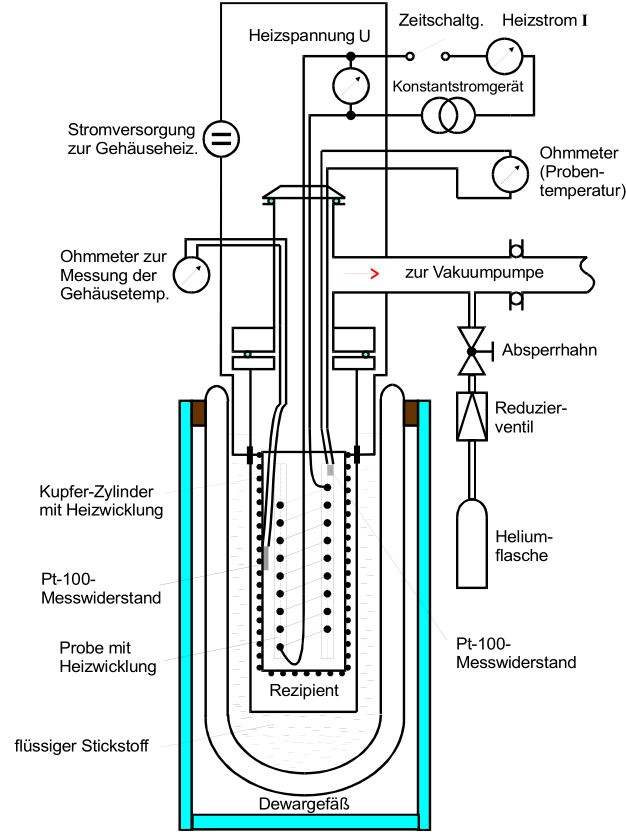
\includegraphics[width = 0.55\textwidth]{Pics/Aufbau.JPG}
  \caption{Schematische Darstellung der verwendeten Messapparatur.}
  \label{fig:Aufbau}
\end{figure}

Zu Beginn des Experimentes wird der Rezipient mithilfe der Vakuumpumpe evakuiert.
Anschließend wird über die Heliumflasche Helium in den Rezipienten geleitet und das
umliegende Dewar-Gefäß mit Stickstoff gefüllt, um die Probe sowie der Kupferzylinder
auf eine Temperatur von $\SI{80}{K}$ abzukühlen. Durch das Helium kann verhindert
werden, dass sich innerhalb des Rezipienten verschiedene Bestandteile der Luft
verflüssigen oder kristalliesieren. Sobald die Probe und der Zylinder auf $\SI{80}{K}$
abgekühlt sind, wird das Ventil zur Vakuumpumpe wieder geöffnet und der Rezipient
erneut evakuiert. Anschließend werden langsam die Temperatur der Probe und des
Zylinders erhöht. Dafür wird bei dem Konstantstromgerät der Heizwicklung für die
Probe ein Strom von $\SI{150}{mA}$ eingestellt. Bei der Heizwicklung des Zylinders
wird der Strom so variiert, dass sich Probe und Zylinder möglichst auf der gleichen
Temperatur befinden. Die Temperatur wird anschließend bis zu einer Endtemperatur
von $\SI{300}{K}$ erhöht. Dabei werden im Abstand von $\SI{5}{K}$ die beiden Widerstände,
die Spannung und der Strom der Probenheizwicklung sowie die vergangene Zeit notiert.
